%\documentclass[12pt, preprint]{aastex}
\pdfoutput=1
\documentclass[floatfix]{emulateapj}
\usepackage{amsmath, xcolor}
\usepackage[boxed]{algorithm2e}
\usepackage{algorithmic}
\usepackage{enumerate}
\usepackage{epsfig,subfigure,color,amsmath,graphicx,multirow,subfigmat,ctable,bm}
\usepackage{natbib}
\newcommand{\rhat}{\hat{\bf r}}
\newcommand{\beq}{\begin{equation}}
\newcommand{\eeq}{\end{equation}}
\newcommand{\beqs}{\begin{eqnarray}}
\newcommand{\eeqs}{\end{eqnarray}}
\newcommand{\R}{{\mathbf R}}
%\floatname{algorithm2e}{Procedure}
\renewcommand{\algorithmicrequire}{\textbf{Input:}}
\renewcommand{\algorithmicensure}{\textbf{Output:}}
\newcommand{\norm}[1]{\left\lVert#1\right\rVert}
\input{epsf} 
\newcommand{\bfi}{\begin{figure}

\end{figure} \epsfxsize=8cm \epsffile}
\newcommand{\efi}{\end{figure}} 
\newcommand{\blankpage}{
\newpage
\thispagestyle{empty}
\mbox{}
\newpage
}
\usepackage[breaklinks,colorlinks,
   urlcolor=blue,citecolor=blue,linkcolor=blue,hyperfootnotes=true]{hyperref}
\usepackage{titlesec}
\usepackage{titletoc}
\usepackage[titletoc, title]{appendix}
%\titleformat{\section}
%{\normalfont\normalsize\bfseries}{\thesection}{1em}{}

%------------------------------------------------------


\begin{document}


\title{{Component separation with conditional generative adversarial networks}}
\author{
$^{1}$ Department of Astronomy, Shanghai Jiao Tong University, Shanghai, 200240, China\\}
\begin{abstract}
In this study, we apply the generative adversarial network (GAN) method to the foreground removal of CMB problem. The results show


\end{abstract}

\keywords{Cosmology: cosmic background radiation, techniques: image processing, method: data analysis}

\maketitle


\section{Introduction}
The cosmic microwave background (CMB) is one of the most powerful cosmological probes to study the physical processes that occurred in the early universe. 

\underline{B mode polarization of CMB}

Regarding the component separation problem, a great deal of work has been carried out in the literature. ???

In the context of CMB, 

Recently, deep learning techniques begin to flourish widely in diverse astronomy fields as soon as they have been proven to be most powerful in computer vision and other scientific areas, with the availability of much faster hardware and larger datasets. In particular, a new charming kind of generative model called generative adversarial networks (GANs) proposed by \cite{2014arXiv1406.2661G} has drawn great attention which can generate fantastic results that even we, human beings, can hardly distinguish from the fake ones.

Generative adversarial networks, as the name suggests, generally can be divide into two parts: $\it{generator}(G)$ and $\it{discrimator}(D)$. With the input of random noise, denoted as $z$, or some signals with  specific distribution, $x + z$, G is responsible for generating imitative images, such as galaxies images with certain shapes, or the sky maps of CMB that have almost the same statistical distributions with the realistic ones, $y$. This generating process is under the supervision of the adversarial part, D. 

???At the beginning, equipped with the expert knowledge of real images, the $\it{D}$ can easily find out the fake images produced by the $\it{G}$ for the latter can hardly understand what is the case. As the training process proceeds, $\it{G}$ start to figure out some rules behind the  ground-truth images and begin to make sense with the feedback of the $\it{D}$, like a layman gradually picks out the correct pictures that present a weak lensing phenomenon. Meanwhile, the discrimator also learn the high-level skills to dig out the fake images. At the convergence point, by virtue of the fighting process, these two counterparts have the same magnitude of power that $\it{G}$ can finally generate images as realistic as possible. This kind of framework can be viewed as a minimax two-player game \citep{2014arXiv1406.2661G},  which can be mathematically expressed by the loss function, Eq.~\ref{cGAN_loss}.

Some attention begin to be paid on the application of GAN to the astronomy fields. 
\cite{2018arXiv181010098R} apply GAN to deblend the target galaxies from two overlapped galaxies, which can be helpful for the pre-process of the data. \cite{2018arXiv181103081F} generate high-resolution synthetic galaxies with some variation of GAN, called chained GAN, to benefit the calibration of shape measurements in the future survey. \cite{2018ComAC...5....4R} propose that GANs can be used to produce realistic samples of cosmic web with a rather faster speed than traditional methods. 

The particular interest in the case of CMB component separation problem is the clean CMB signal hided behind the complicated total microwave signal, which can be seen as a translation from the observed sky maps to the pristine CMB anisotropies, in pixel space. Particularly, \cite{2016arXiv161107004I} proposed a kind of framework called $\it{pix2pix}$ based on conditional GANs (cGAN) to do the \underline{image-to-image transformation such as transforming }the day scene pictures to the night ones. 

????Here, we report the results of CMB component separation using a machine learning model on the basis of cGAN model ...???? . 

The paper is organized as follows. In Sect.~\ref{sect:network}, we briefly review the GAN approach and introduce the architecture of our model. Sect.~\ref{sect:maps} introduces our simulated maps and we present the application of the GAN to the simulated skies in Sect.~\ref{sect:test}. Finally, we draw our conclusions in Sect.~\ref{sect:con}.

\section{Network architecture(a figure)}\label{sect:network}
The standard GAN itself is recognized as a kind of unsupervised learning for that we only need to label out the real data at the initial phase without further human intervention, that is $G: z\rightarrow y$. Conditional GAN, however, in which $\it{G}$ knows the corresponding ground-truth images that it mimics, can be classified into supervised learning, $G: \{x,z\}\rightarrow y$.

\underline{Here is needed to be described more carefully...}
\begin{figure*}[htpb]
\centering
\mbox{
 \subfigure{
   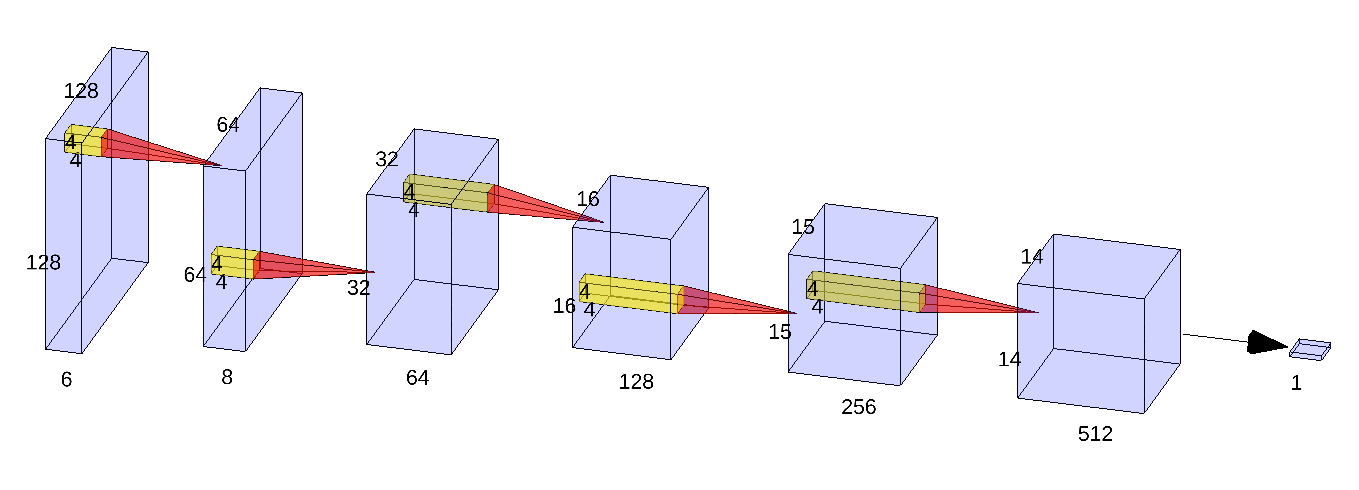
\includegraphics[width=7.0in] {fig/arch_D.png}
   }
}

\caption{The architecture of the discriminator. The yellow cube represents the convolution method with a kernel of 4*4 pixels and the red cone stands for the activation function....................... }
\label{fig:arch_D}
\end{figure*}

\begin{figure*}[htpb]
\centering
\mbox{
 \subfigure{
	 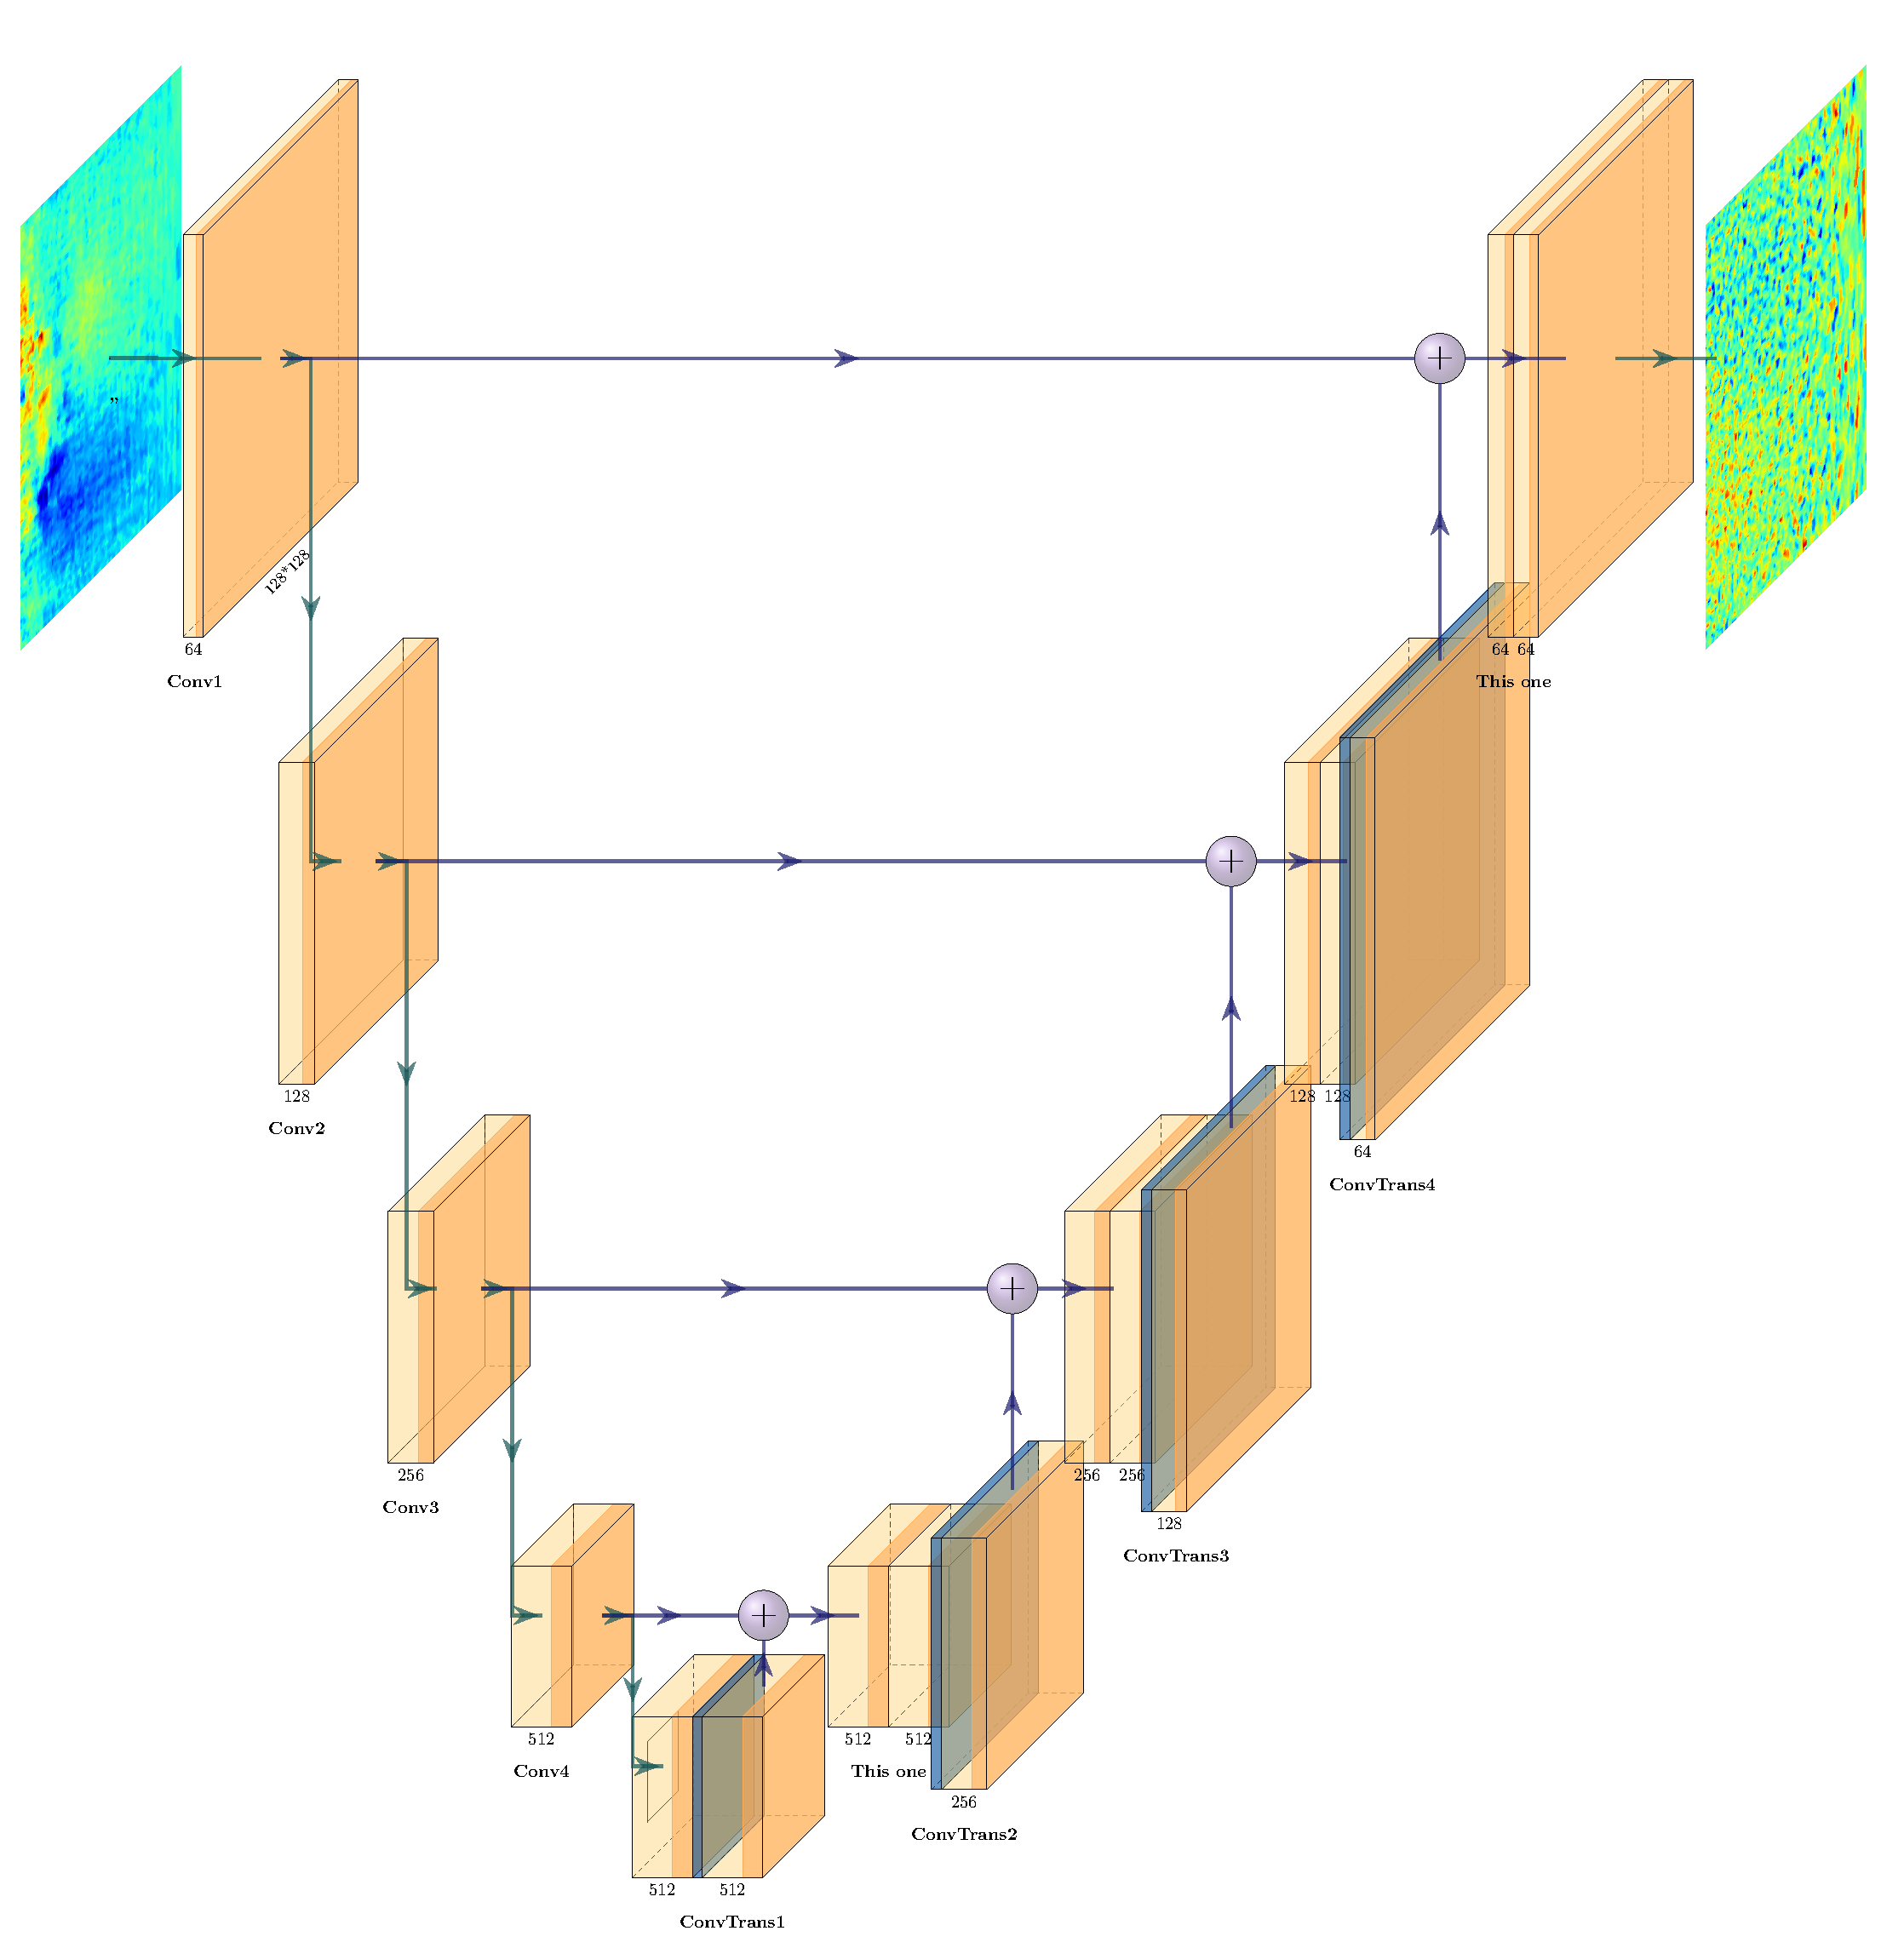
\includegraphics[width=6.0in, height = 5in] {fig/Unet_ushape.pdf}
   }
}

\caption{The architecture of the generator. Non-linear activation brings non-linearity into the network. }
\label{fig:arch_G}
\end{figure*}

\subsection{Loss function}\label{sect:loss}

A $\it{Loss\ function}$ is applied beyond the neural networks to reveal the instaneous error between the output and corresponding ground truth, which should be as small as possible. With the error in mind, the networks can do self-examination, usually armed with gradient descent techniques, to find the correct direction to reach the optimal point in the parameter space. It may have various mathematical expressions, like mean square error($\it{MSE}$) usually applied in regression tasks or cross entropy often used in classification problems.

For cGAN, the loss function  explicitly describes the fighting process between the competitors. 

\begin{align}\label{cGAN_loss}
    \mathcal{L}_{cGAN}(G,D) = &\mathbb{E}_{x,y}[\log D(x,y)] + \nonumber \\
                 &\mathbb{E}_{x,z}[\log (1-D(x,G(x,z))],\
\end{align}
where the $\mathbb{E}$ is the expectation value over the training set.

In Eq.~\ref{cGAN_loss}, $D$ tries to maximizing the loss function, preventing $G$ from minimizing it by giving the real pairs, $\{x,y\}$, high credits, while lowering the ones of fake pairs: $\{x, y_{fake} = G(x,z)\}$. Our hope, $G$, will learn to mess the $G$ around to increase its grades and minimize the loss. So our objective is to get $G^*  = \arg\min_G \max_D \mathcal{L}_{cGAN}(G,D)$.

The $pixpix$ model also includes the L1 loss which tells the pixel-wise differences between the fake pictures and the real ones, so that $G$ will also try to generate the output near the ground truth rather than just circling around with the discriminator:
\begin{equation}
\begin{split}
    \mathcal{L}_{L1}(G) = &\mathbb{E}_{x,y,z}[\norm{y-G(x,z)}_1] \\
    =&\frac{1}{mn}\sum_{i=1}^{m} \sum_{j=1}^{n} {[y_{CMB}^{(i,j)} - x_{CMB}^{(i,j)}]^2}, \label{L1_equation} 
\end{split}   
\end{equation}
where m,n is the number of row and column pixels in the pictures and $y_{CMB}^{(i)}$ and $x_{CMB}^{(i)}$ represent the value of \textit{i}th pixel in the generated maps and the ground-truth, respectively.  
We also tried to use the L2 norm as the loss function and found that it has little impact on the performance.


\subsection{U-net structure}
Besides theoretical research, the engineer-part of machine learning is to design different types of architecture with succeeding fine-tunings and see whether it works. \cite{2015arXiv150504597R} design a kind of network call $Unet$ that the deeper layers can receive some information from shallower layers with direct connection. As the layer becomes deeper, the message it carries becomes more local and delicate. For our component separation tasks, we consider that the shallower layers will learn the large scale structures while the deeper ones can focus on the small scale structures.  So we think that the direct connection between different scales can benefit the recover process. A more illustrative presentation can be found in Fig. \ref{fig:arch_G}. 

When passing through deeper layer in the left part, the input pictures will become 2 times smaller than the previous layer while increasing the channel number due to the $down-sampling$ method that utilize the $convolution$ operation. So the left part can be seen as an $encoder$ which transform the original data into the machine learning language. On the contrary, the right part is like a $decoder$ to bring forth the intentional information back by the $up-sampling$ method.  


\subsection{Activation function}
An activation function is always presented at the end of the network to perform a non-linear mapping of the output, which in turn defines the input of the next node. One of the commonly used activation functions is called Rectified Linear Unit (ReLU), expressed as f($x$) = max($x$, 0). For the discrimator and the \underline{encoder} (down-sampling) part, we use the ordinary ReLU and for the \underline{decoder}(up-sampling) part we add a slope of 0.2 for the smaller-than-zero part which reads:

\begin{equation}
f(x) = 
\begin{cases}
	0.2x\quad  &if \quad x < 0 \\
	x   \quad  &if \quad x \geq 0
\end{cases}
\end{equation}
\subsection{Network}
For each training sample, we place the total signal that consists of the pure CMB and some foreground signals at the upper part of the whole image and the same CMB realization at the lower part, as the ground truth. That is to say one sample includes a pair of maps --- total signal is the input, the clean CMB map is the output of the network. 

For polarization, we use Stokes Q and U maps as the input CMB maps and concate the 3 frequencies, between which CMB polarization maps are the same due to the thermal blackbody spectrum of CMB while the foregrounds are frequency-dependent, to have 6 channels in total as input. These input maps are shown in Fig.~\ref{fig:input_maps}. We set the output as two channels to have clean Q and U maps. Then we use the $anafast$ routine of HealPix \citep{2005ApJ...622..759G} to calculate the E and B mode signals from the Q and U polarization. 

\begin{figure*}[htpb]
\centering
\mbox{
 \subfigure{
   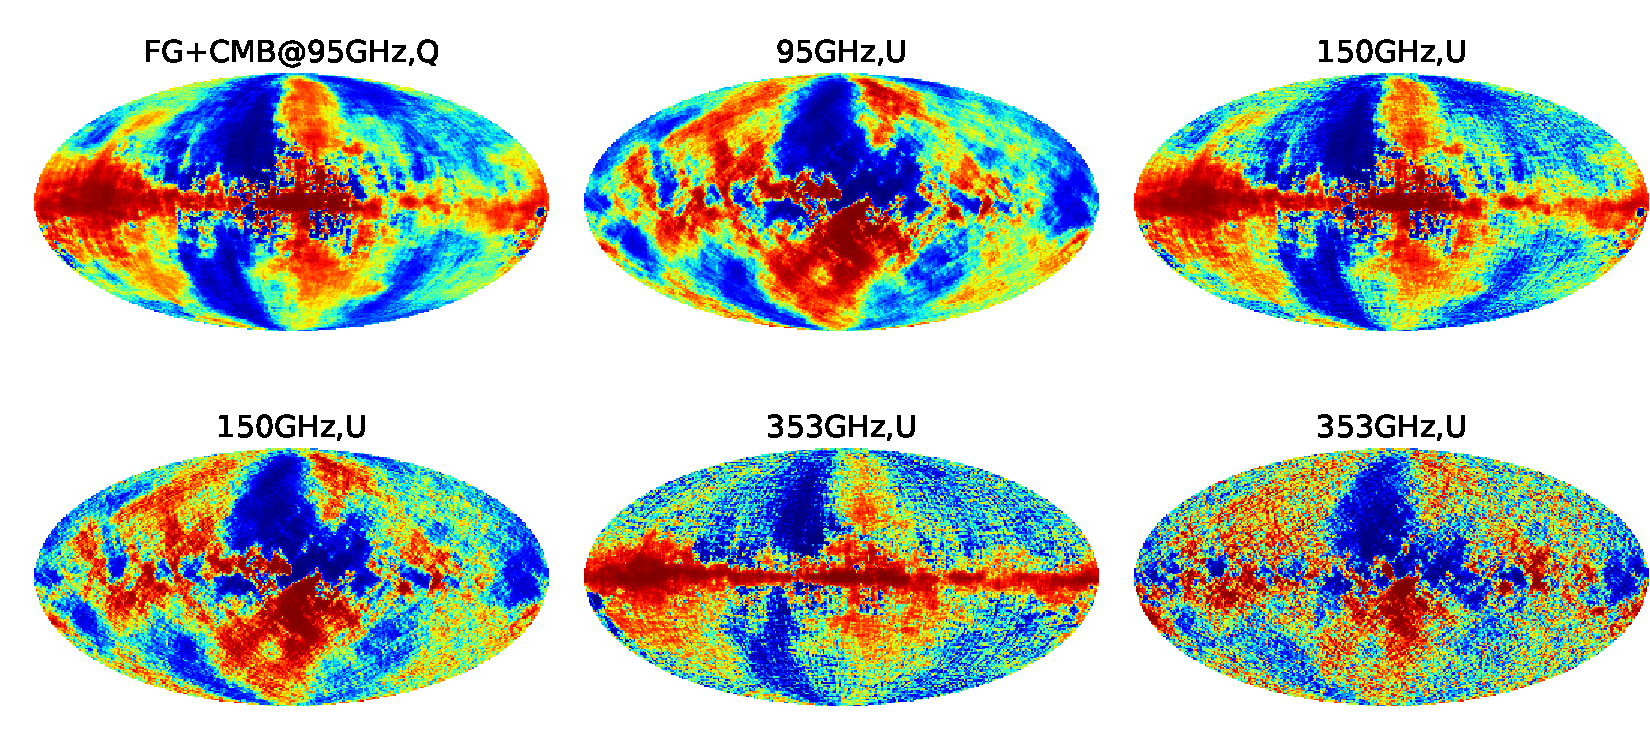
\includegraphics[width=7.0in] {fig/Input_total_maps.pdf}
   }
}
	
\caption{The inputs maps of the network.}
\label{fig:input_maps}
\end{figure*}

\subsection{To avoid overfitting}
batch normalization 
\subsection{Evaluation}
To evaluate the results obtained by the network, we propose two kinds of measurement tests: one is in the pixel space and the other is in harmonic space.
 
To quantify the similarity between the reconstructed and input CMB maps, we adopt the Pearson's correlation coefficient:  
\begin{align}
\rho(y,x) = \frac{\sum_{i=1}^{n} [y^{(i)} - \overline{y}^{(i)}][x^{(i)} - \overline{x}^{(i)}]}{\sum_{i=1}^{n}[y^{(i)} - \overline{y}^{(i)}]^2 \sum_{i=1}^{n}[x^{(i)} - \overline{x}^{(i)}]^2},
\end{align}
where $\overline{y}$ and $\overline{x}$ represent the mean values of $y_{CMB}$ and $x_{CMB}$.

And to determine the accuracy of the recovered power spectrum compared to the input B-mode, we re-project the plane maps back to the sphere and calculate the tensor signal.
\section{Test on the simulated maps}\label{sect:maps}

For deep learning models to fully work, it is required and important to get big(number) and well-designed datasets.

\subsection{Simulated datasets}
  
We consider synchrotron, dust and anomalous microwave emission (AME) as polarized foreground components and we also add \underline{Ali-level} white noise to validate our tests. 
We generate the $Planck$-like maps as training datasets at 95, 150 and 353 GHz using different foreground models provided by the package \texttt{Pysm} \citep{2017MNRAS.469.2821T}. 

For synchrotron, they model the polarization as a scaling of the WMAP 9-year 23 GHz Q and U maps \citep{2013ApJS..208...20B}, smoothed to three degrees and parameterize the spectral index to be a power-law in each direction. The nominal model for thermal dust polarization uses template maps at 353GHz smoothed to two degrees FWHM, which is estimated from the $Planck$ data using the ‘Commander’ code and the frequency scaling is treated as a signal component. AME is thought to be slightly polarized \citep{2011MNRAS.418L..35D} and the model sets the global polarization fraction as 2\% on the basis of Planck templates.

\underline{To change the amplitude of CMB tensor, we use camb} $\footnote{\url{https://camb.info/}}$ ,,,,,,,,,,,
\cite{Lewis2000} with the standard \underline{Planck cosmological parameters}. 
To be more realistic, we also add the instrumental noise that is independent between different scales and frequencies. 
	
Fig.~\ref{fig:fg_tensor} shows the B-mode power spectrum of different foreground model combination at 95 GHz. 
\begin{figure*}[htpb]
\centering
\centering
\mbox{
 \subfigure{
	 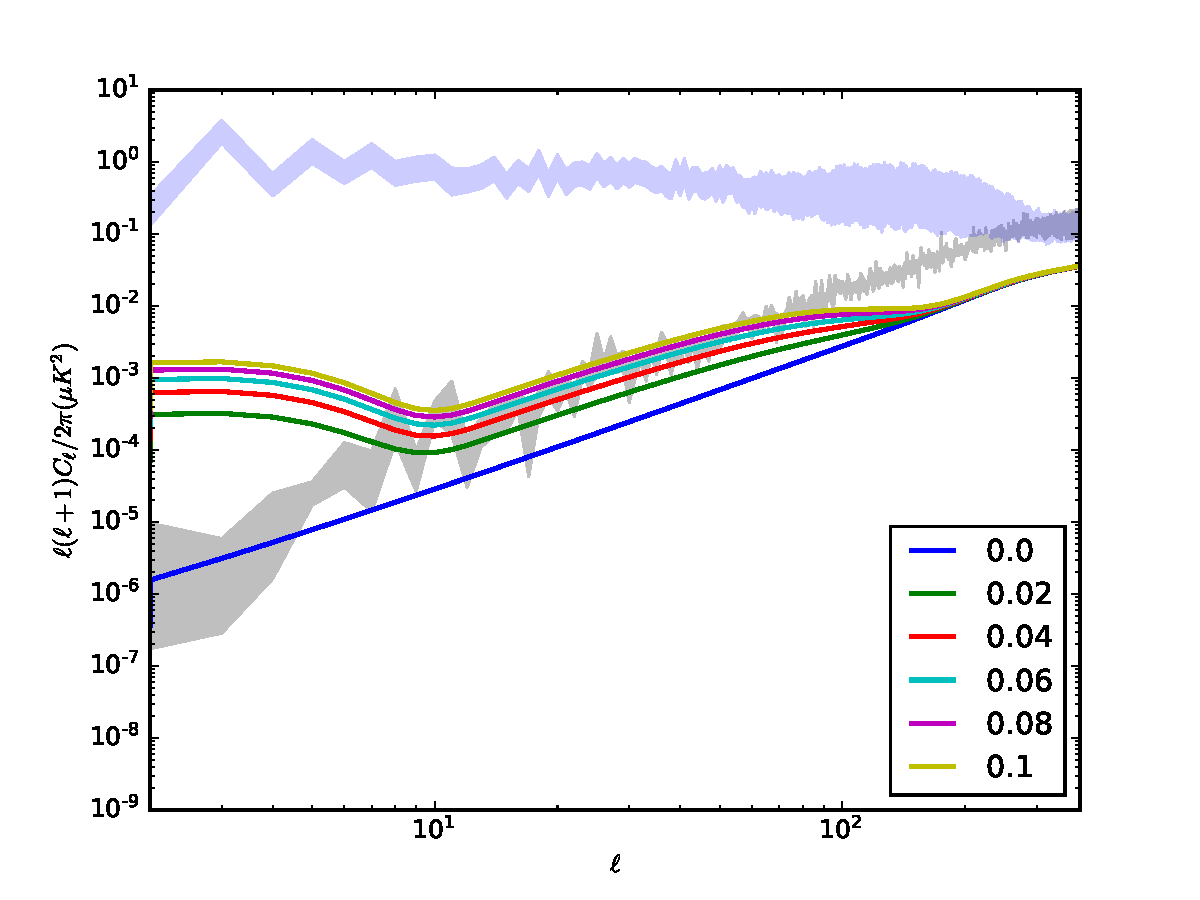
\includegraphics[width=3.8in] {fig/B_mode_signal.pdf}
   }

 \subfigure{
   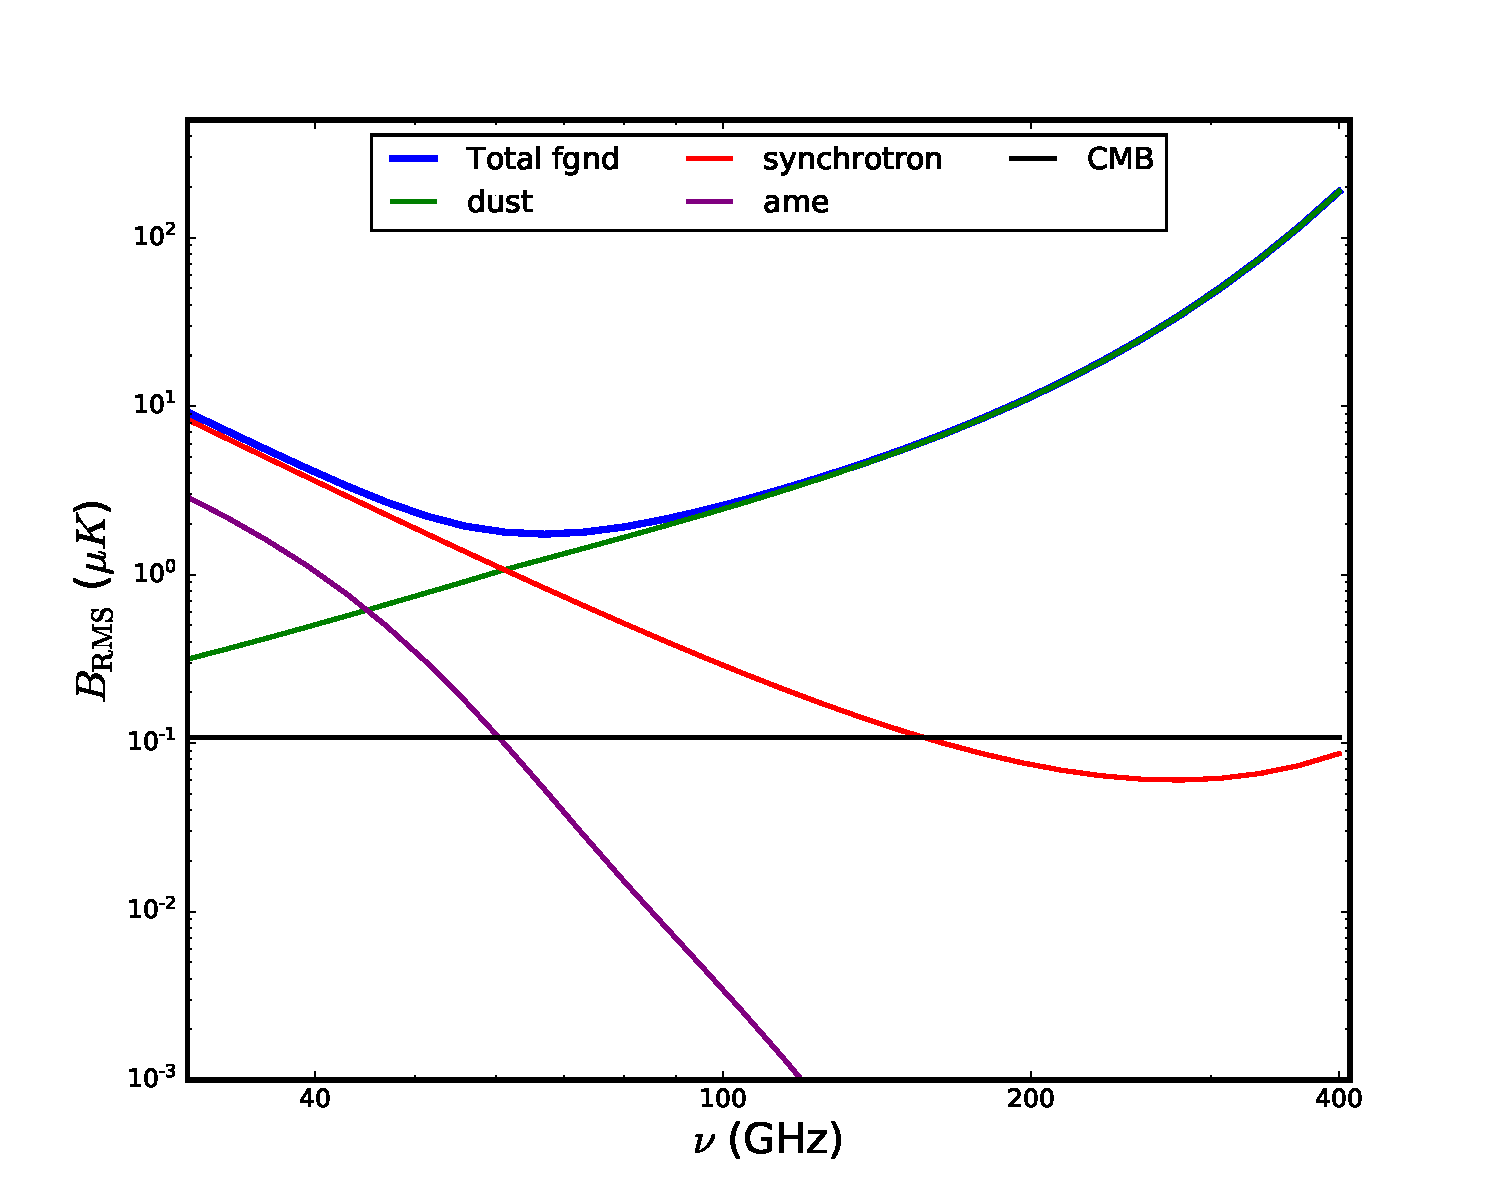
\includegraphics[width=3.6in] {fig/foreground_rms.pdf}
   }
}
 
%\mbox{
% \subfigure{
%   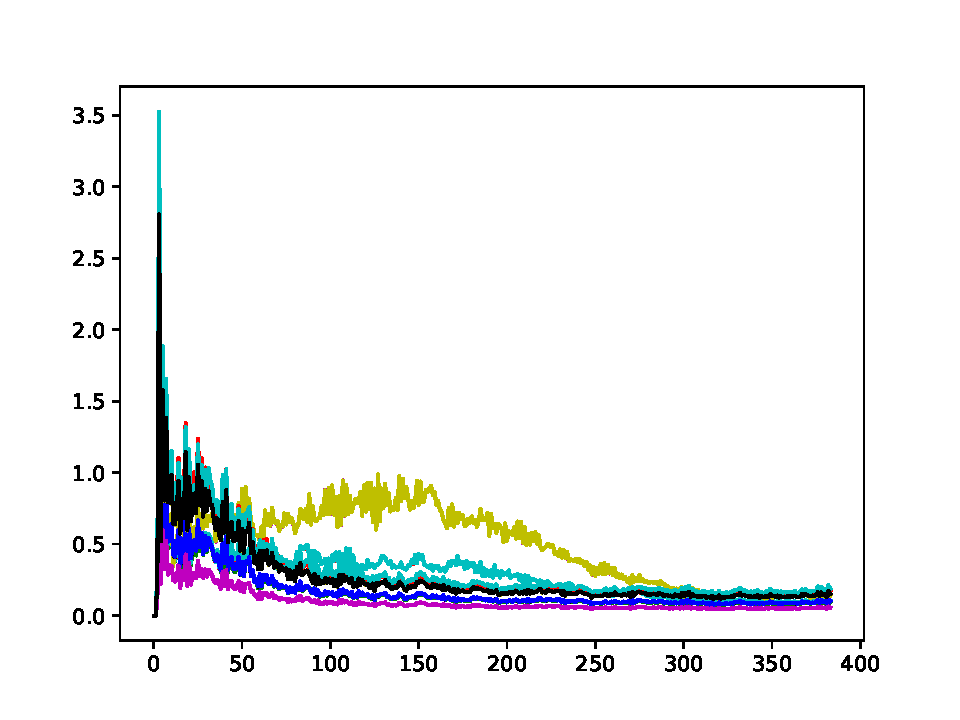
\includegraphics[width=2.3in] {fig/foregrounds_tensor.pdf}
%    }} {\it Upper panels}


\caption{ The B-modes of different foregrounds model in the Pysm package. }
\label{fig:fg_tensor}
\end{figure*}

\subsection{Sphere-to-plane transformation}

With full-sky maps at hand, we then select a small patch of the sky and then convert them into plane format to ease the burden of computation. The sphere-to-plane transformation is a very complicated problem and there many works trying to deal with spherical data commonly in cosmology. \cite{2018arXiv181012186P} develop a spherical convolutional neural network (CNN) called $DeepSphere$ for analysis of full and partial HEALPix maps using the graph-based representation.

For our test, we use plane approximation to represent the sphere data $--$ we simply construct a matrix mesh with 64 by 64 pixels that sampled with equal distance between $\lbrace$RA=(5,85), DEC=(-60,60)$\rbrace$. With the coordinates of each entries of the matrix, we can know exactly its place on the sphere and get its value. Although this kind of projection may lose some useful information, we think that the loss can be viewed as an artificial mask of the map \underline{and we know that the mask only brings the ratio effect.} We then re-project the plane-maps into spherical maps in order to calculate the power spectrum  more conveniently. The sky maps used in our experiments are shown in Fig.~\ref{fig:recovered_maps}.
\begin{figure*}[htpb]
\centering
\mbox{
 \subfigure{
   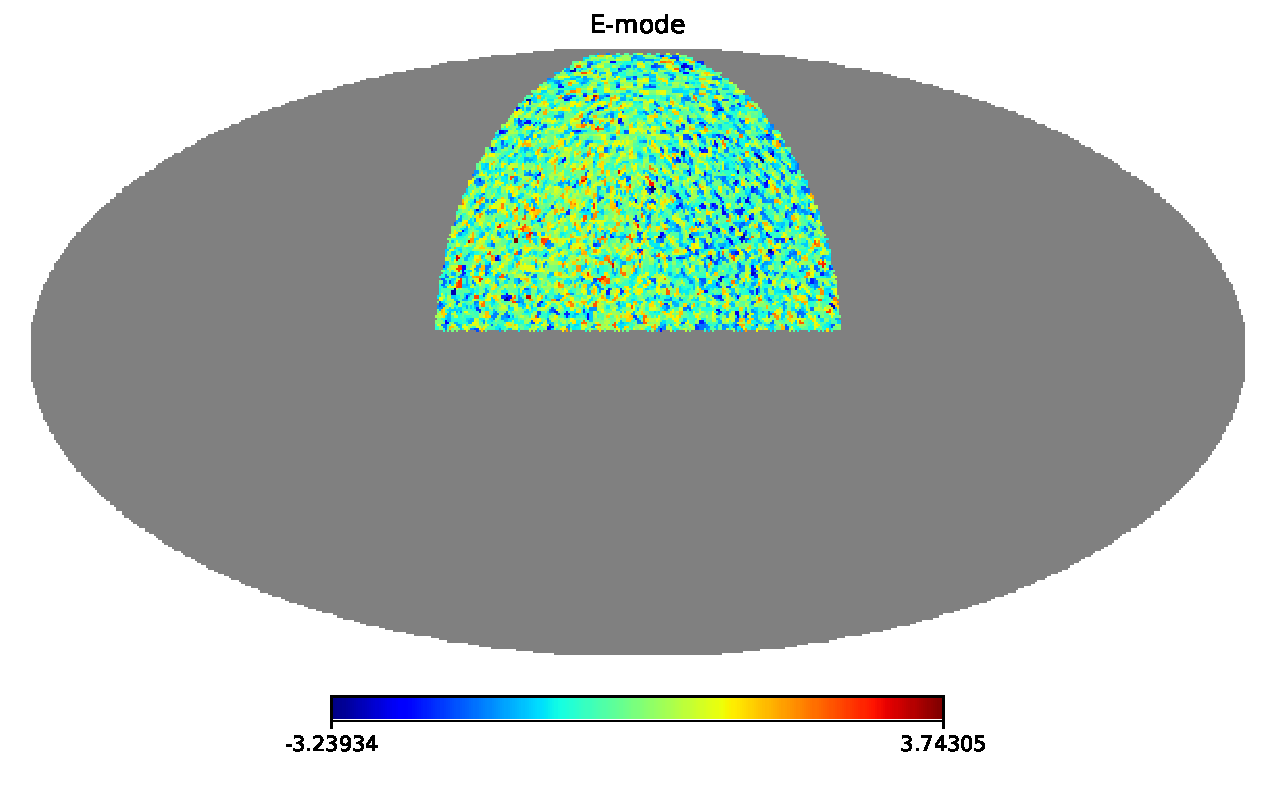
\includegraphics[width=2.3in] {fig/CMB_E-mode.pdf}
   }
\subfigure{
   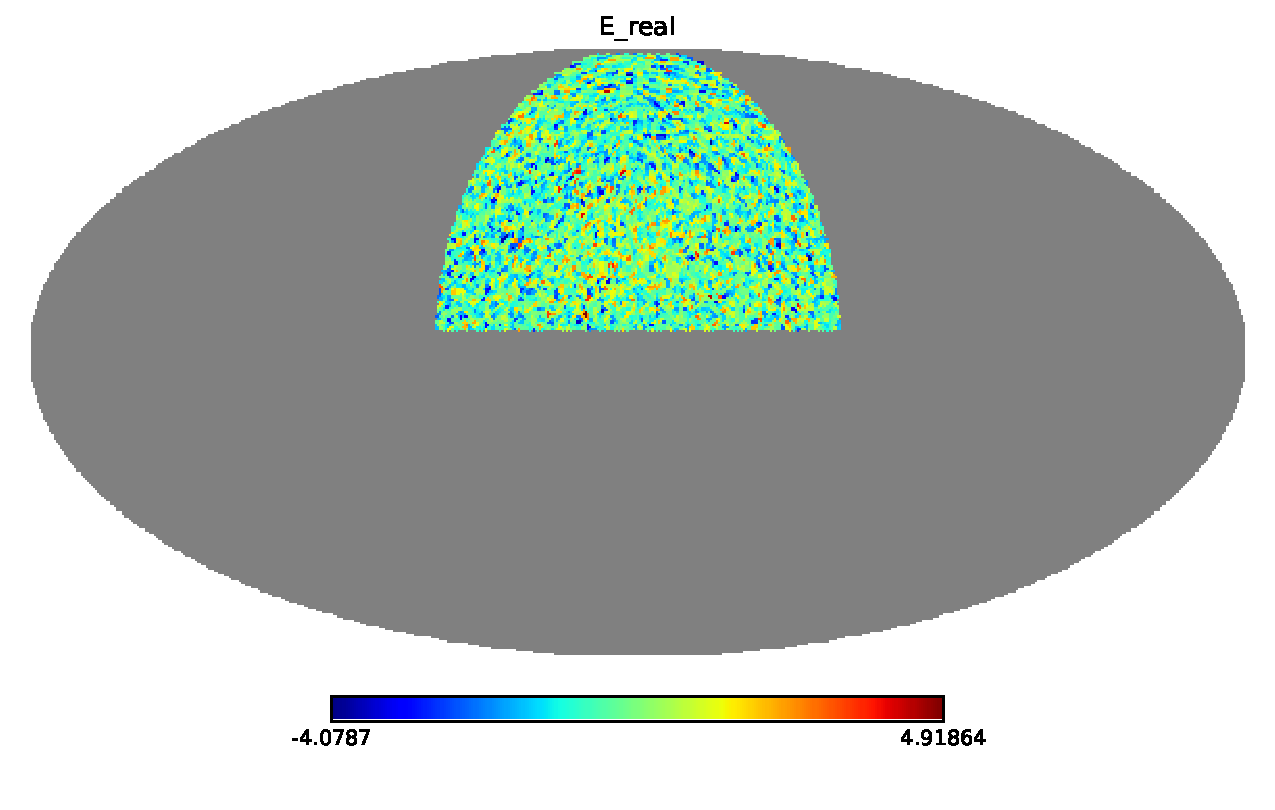
\includegraphics[width=2.3in] {fig/E_real.pdf}
   }
\subfigure{
   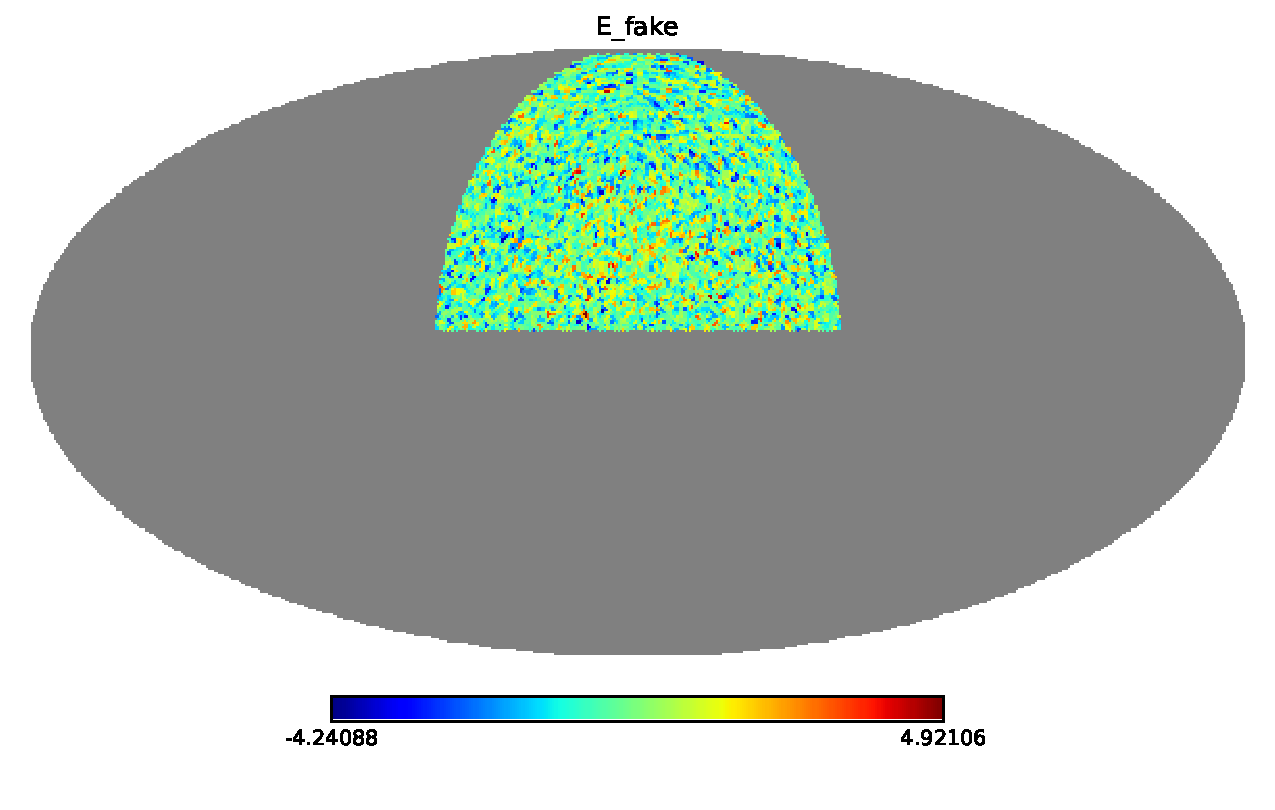
\includegraphics[width=2.3in] {fig/E_fake.pdf}
}}
\mbox{
 \subfigure{
   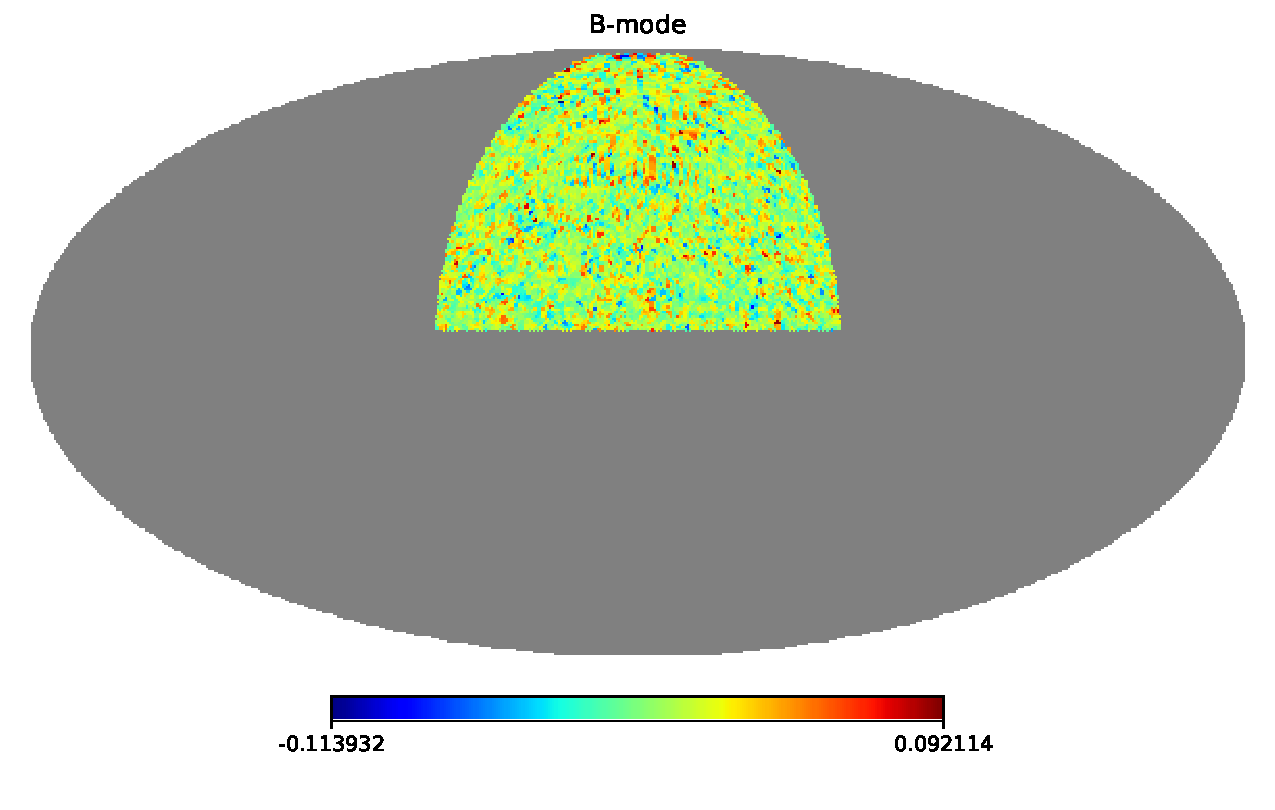
\includegraphics[width=2.3in] {fig/CMB_B-mode.pdf}
   }
\subfigure{
   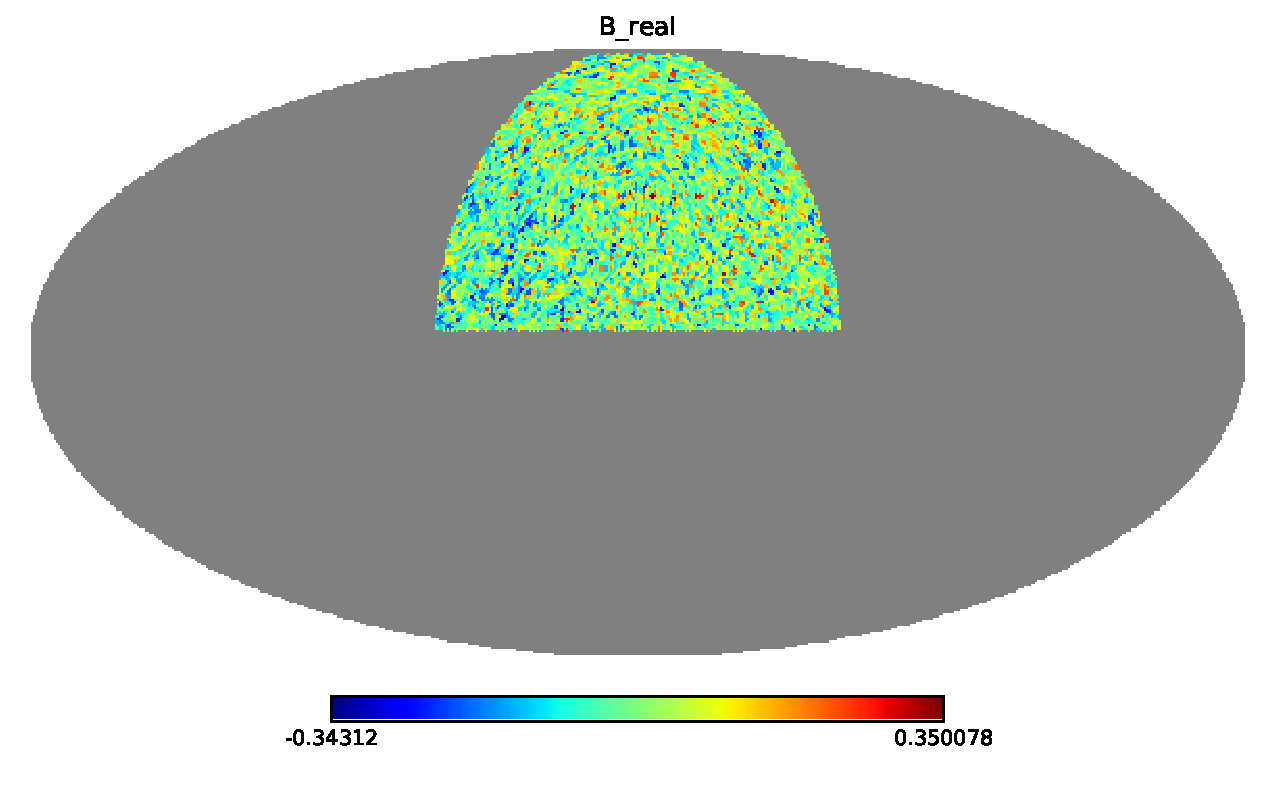
\includegraphics[width=2.3in] {fig/B_real.pdf}
   }
\subfigure{
   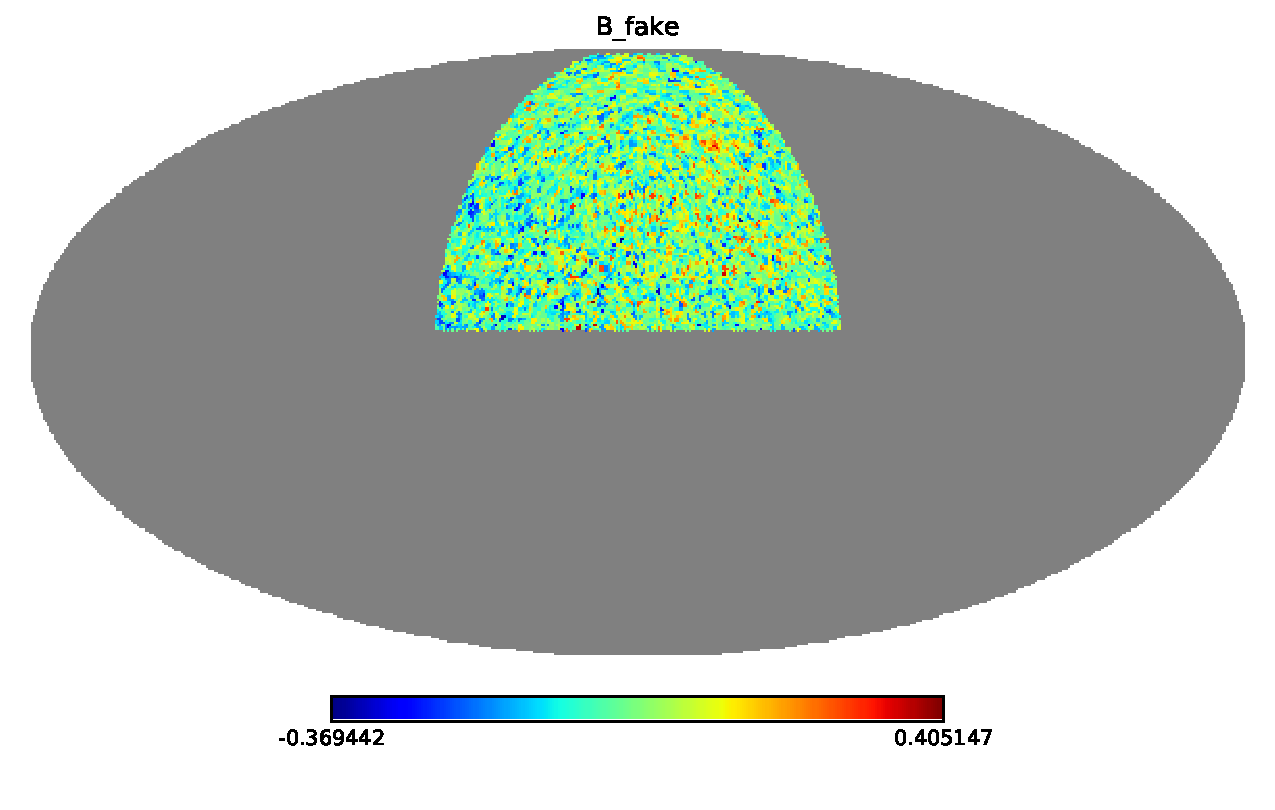
\includegraphics[width=2.3in] {fig/B_fake.pdf}
   }
}
\caption{{\it Left column}: One realization of CMB polarization for E and B modes. {\it Middle column}: The re-projected E and B maps. {\it Right column}: The recovered E and B maps of the network. \textcolor{red}{This should be replaced by plane-projection (that is a square) ..}}
\label{fig:recovered_maps}
\end{figure*}

\subsection{Training data and testing data}
For training data...
We split the simulated database into training samples containing 80\% of the images and the rest 20\% as the test datasets.

For testing data, we use different realization of CMB and random model of foregrounds... The results are shown in the upper panel of Fig.~\ref{fig:recovered_ps}.
 
We can see the B-mode result in the right column shows the expected bump at low $\ell$ due to the well-known E-B leakage problem raised by the masks, while the original B-mode has no this kind of feature. 

Although the E-B leakage problem has been solved well(\underline{References needed}) after years' efforts, we try to let the network learn to discover and solve this tricky thing spontaneously and simultaneously by itself. So we re-design the output maps as E- and B-modes maps in accordance with the input Q and U maps, following below steps:
\begin{enumerate}[(A)]
\item Firstly call the \emph{map2alm} function to get the alms $\{almT, almE, almB\}$. 
\item Then call the \emph{alm2map} funtion to transform the almE and almB  to E and B maps.
\item Last select the patch of the full-sky maps of E and B maps and label the patch as the ground-truth.
\end{enumerate}
 
and the result is the lower panel of Fig.~\ref{fig:recovered_ps}.

For the practical tensor signal, we do not know its exact amplitude or shape. To further improve the generality of the model, we consider several conditions. We change the amplitude by a factor between (0.1, 10), with r = 0.1 as the baseline. (to be determined...) We also artificially set the shape of B-mode power spectrum to be a straight line with the value of .... and for every l we multiply with a random number between (0.1,1). \underline{Figure result need...}



figure that includes the shaded area of different foreground model (!!!)


\begin{figure*}[htpb]
\centering
\mbox{
 \subfigure{
   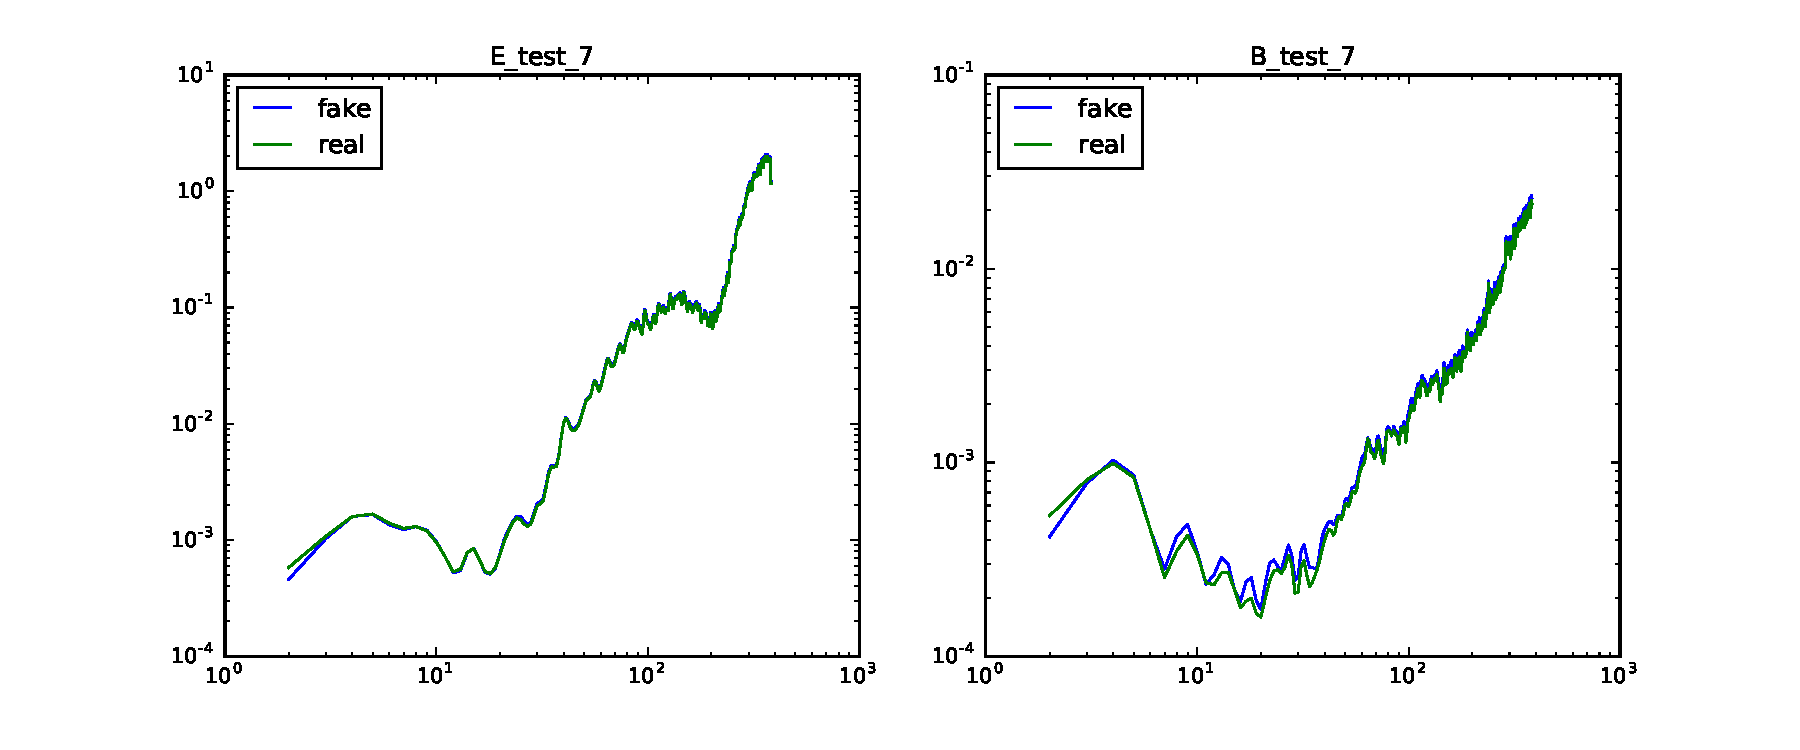
\includegraphics[width=7.0in] {fig/Test_best_1121_noise_ali.pdf}
   }
}

\mbox{
 \subfigure{
   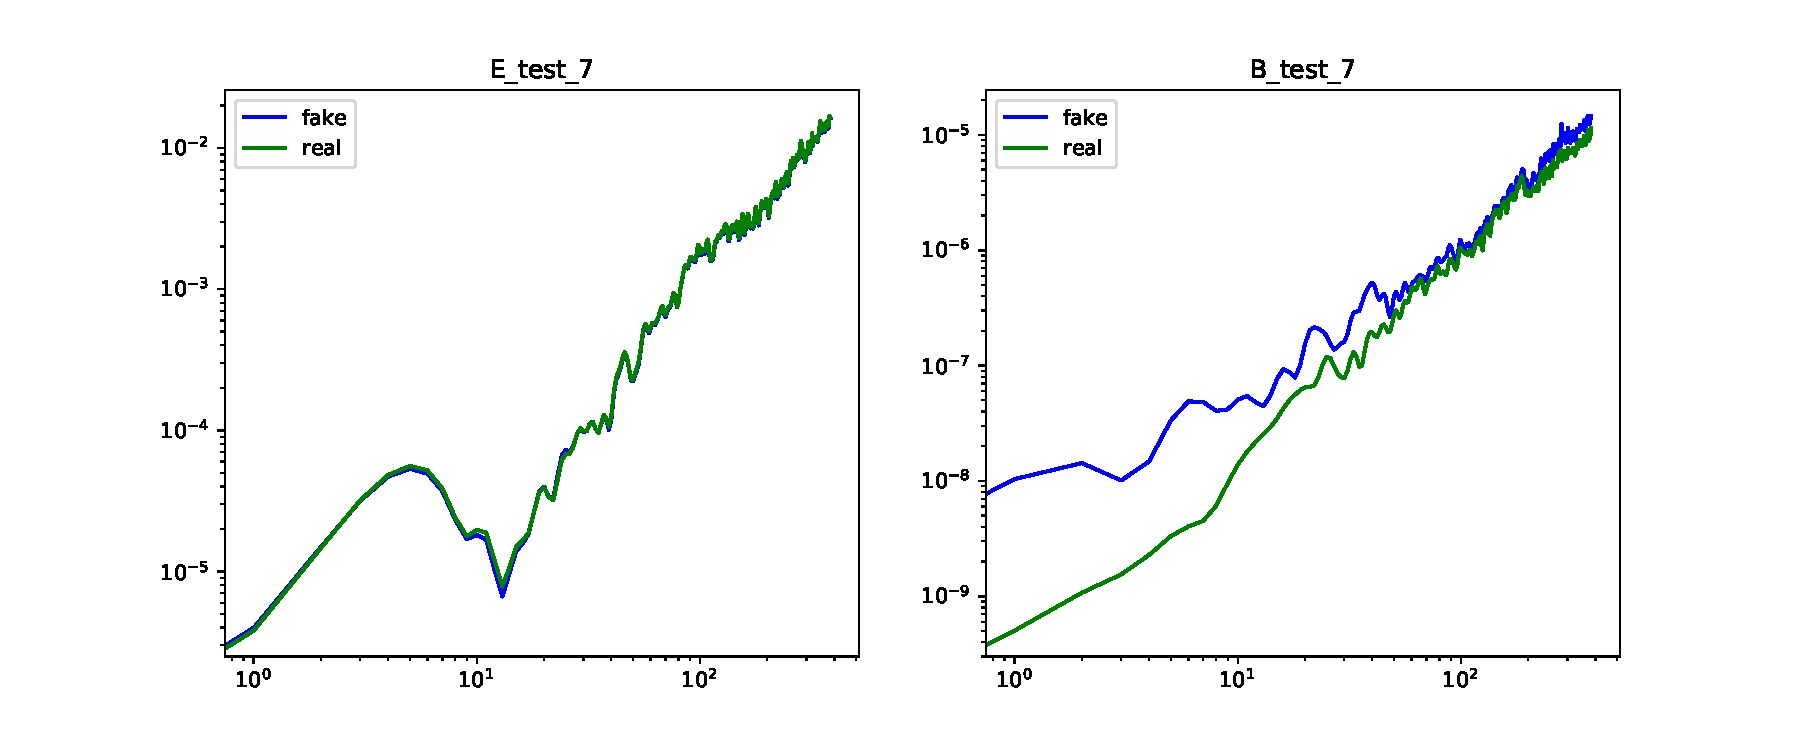
\includegraphics[width=7.0in] {fig/Test_best0104_noisy_353.pdf}
   }

}

\caption{The left columns are E-mode power spectrum and the right ones are B modes. {\it Upper panel}: The results of E- and B-mode power spectrum calculated from the Q- and U-maps recovered by the network. {\it Lower panel}: The E- and B-mode power spectrum from E and B maps recovered by the network.}
\label{fig:recovered_ps}
\end{figure*}

\subsection{Test against different foregrounds with different tensor-to-scalar ratio}
In order to validate the robustness of our network, we perform several test against different foregrounds models by increasing the amplitude of each component within the three kinds. For each combination, we have 50 realization of sky maps from the same $r$ and calculate the mean value and standard deviation of these realization and further test with different $r$ values.
\section{Conclusions}\label{sect:con}
We have 
\underline{The results show a great dependence} on the foreground models which rely on the complete understanding about the complicated foregrounds... If we have better and more realistic modelling on the structure about the spining dust, then we will have more properties to be learned by the neural networks, which will benefit the generality of the networks.

We have struggled with the projection process, trying to preserve all the pixel information............ 

The weightting method has made the target output Q and U maps of different frequencies not identical, differing with a factor, and we have given hope to the network to recognize this factor automatically which was not necessarily precise.

We can use the power spectrum as the output of our network for future work.
In the future, we want to generalize to ,,, with this we hope to ...

We argue that machine learning can be tuned to have great power to solve many non-trivial problems much better than, at least at the same level as human beings. But we just use it as a almighty tool without knowing the sense behind it. When this kind of black box works well, we are excited to regard ourselves as super-master of smart androids; when it strikes, we almost have nothing to do except re-designing the androids. How to understand the behaviour of neural networks really needs to call for attention...
\section*{Acknowledgements}

\begin{appendices}
%\vspace{-1.5em}

\section{Experiment details}
We use the open-source python library, Pytorch $\footnote{Pytorch: \url{https://pytorch.org/}}$ as the implementing framework and speed up the learning process on the Tesla-k40 GPUs with the help of CUDA toolkit $\footnote{CUDA: \url{https://developer.nvidia.com/cuda-toolkit}}$, which is commonly utilized in the machine learning fields.



In our experiments, we also weight different frequencies with the ratio of their variance respect to the highest frequency, i.e., 353GHz. we found that if we use 3 frequencies and treat each frequency equally, the results would be not satisfactory. Note that if we weight each frequency with their variance, then ground-truth, i.e., pure CMB signal, pertaining to the input would become different with each other, with a norm factor. Then the output should  be not 2 channels but 6 channels. But we still use 2 channels of the first frequencies as the output for brevity. 


To further assess and validate ...

\end{appendices}

\bibliographystyle{aasjournal}

\begin{thebibliography}{99}

\bibitem[Bennett et al.(2013)]{2013ApJS..208...20B} Bennett, C.~L., Larson, D., Weiland, J.~L., et al.\ 2013, The Astrophysical Journal Supplement Series, 208, 20.

\bibitem[Dickinson et al.(2011)]{2011MNRAS.418L..35D} Dickinson, C., Peel, M., \& Vidal, M.\ 2011, \mnras, 418, L35.

\bibitem[Fussell, \& Moews(2018)]{2018arXiv181103081F} Fussell, L., \& Moews, B.\ 2018, arXiv e-prints , arXiv:1811.03081.

\bibitem[G{\'o}rski et al.(2005)]{2005ApJ...622..759G} G{\'o}rski, K.~M., Hivon, E., Banday, A.~J., et al.\ 2005, \apj, 622, 759

\bibitem[Goodfellow et al.(2014)]{2014arXiv1406.2661G} Goodfellow, I.~J., Pouget-Abadie, J., Mirza, M., et al.\ 2014, arXiv:1406.2661 
\bibitem[Isola et al.(2016)]{2016arXiv161107004I} Isola, P., Zhu, J.-Y., Zhou, T., et al.\ 2016, arXiv e-prints , arXiv:1611.07004.

\bibitem[{Lewis {et~al.}(2000)Lewis, Challinor, \& Lasenby}]{Lewis2000} Lewis, A., Challinor, A., \& Lasenby, A. 2000, \apj, 538, 473

\bibitem[Perraudin et al.(2018)]{2018arXiv181012186P} Perraudin, N., Defferrard, M., Kacprzak, T., et al.\ 2018, arXiv e-prints , arXiv:1810.12186.

\bibitem[Reiman, \& G{\"o}hre(2018)]{2018arXiv181010098R} Reiman, D.~M., \& G{\"o}hre, B.~E.\ 2018, arXiv e-prints , arXiv:1810.10098.

\bibitem[Rodr{\'\i}guez et al.(2018)]{2018ComAC...5....4R} Rodr{\'\i}guez, A.~C., Kacprzak, T., Lucchi, A., et al.\ 2018, Computational Astrophysics and Cosmology, 5, 4.

\bibitem[Ronneberger et al.(2015)]{2015arXiv150504597R} Ronneberger, O., Fischer, P., \& Brox, T.\ 2015, arXiv e-prints , arXiv:1505.04597.


\bibitem[Thorne et al.(2017)]{2017MNRAS.469.2821T} Thorne, B., Dunkley, J., Alonso, D., \& N{\ae}ss, S.\ 2017, \mnras, 469, 2821

%\bibitem[Yao et al.(2018)]{2018ApJS..239...36Y} Yao, J., Zhang, L., Zhao, Y., et al.\ 2018, \apjs, 239, 36 
%\bibitem[Zhang et al.(2016)]{2016arXiv160803707Z} Zhang, P., Zhang, J., \& Zhang, L.\ 2016, arXiv:e 


\end{thebibliography}

%\bibliography{le}
%\bibliographystyle{apj}
%\nocite{*}



\end{document}



